
\documentclass[11pt]{beamer}
\usepackage{helvet} %font
\beamertemplatenavigationsymbolsempty
\usetheme{JuanLesPins}
\usefonttheme{structurebold}

\usepackage[french]{babel}
\usepackage[utf8]{inputenc}
\usepackage[T1]{fontenc}
\usepackage{amssymb,amsmath}
\usepackage{tikz}
\usepackage{geometry}
\usepackage{xcolor,colortbl}
\usetikzlibrary{arrows,positioning}
\usepackage{listings}

\AtBeginSubsection[]
{
   \begin{frame}
	\small \tableofcontents[currentsection]
   \end{frame}
}

\newenvironment{slide}[1]{%
\begin{frame}[environment=slide]
\frametitle{#1}
}{%
\end{frame}
}
\setbeamercolor{structure}{fg=red}
\setbeamercolor{frametitle}{bg=black,fg=white}
\definecolor{gris}{gray}{0.6}
\definecolor{grisclair}{gray}{0.9}

\newtheorem{exercice}{Exercice}

\title{Machine Learning III \\ Introduction à \texttt{scikit-learn}}
\author{Nicolas Bourgeois}
\date{}

\newcommand{\Python}[1]{
	{\small	\lstinputlisting[language=Python]{./#1.py}}
}
\newenvironment{pyenvsmall}
	{ \ttfamily \tiny }
	{\par  }

\newcommand{\Pythonsmall}[1]{
	{\scriptsize \lstinputlisting[language=Python]{./#1.py}}
}
\newcommand{\elimine}[1]{{\textcolor{lightgray}{#1}}}

\newcommand\Wider[2][3em]{%
\makebox[\linewidth][c]{%
  \begin{minipage}{\dimexpr\textwidth+#1\relax}
  \raggedright#2
  \end{minipage}%
  }%
}

\begin{document}

\begin{frame}
\maketitle
\end{frame}

\begin{frame}{Télécharger}

Data and Cheatsheets :\\
\vspace{0.3cm}

\url{ouralou.fr/Resources/epita/C3.zip}


\end{frame}


\begin{frame}{Exercice}
\begin{exercice}
Importez les données de data1.csv et testez une régression linéaire entre la longueur et l'épaisseur des pétales.
\end{exercice}
\begin{exercice}
Même question, cette fois entre la longueur des cépales et la largeur des pétales. Comparez les scores des deux régressions.
\end{exercice}
\begin{exercice}
Dans les deux cas, représentez les données et la droite de régression.
\end{exercice}
\end{frame}

\begin{frame}{Résultat attendu (1)}
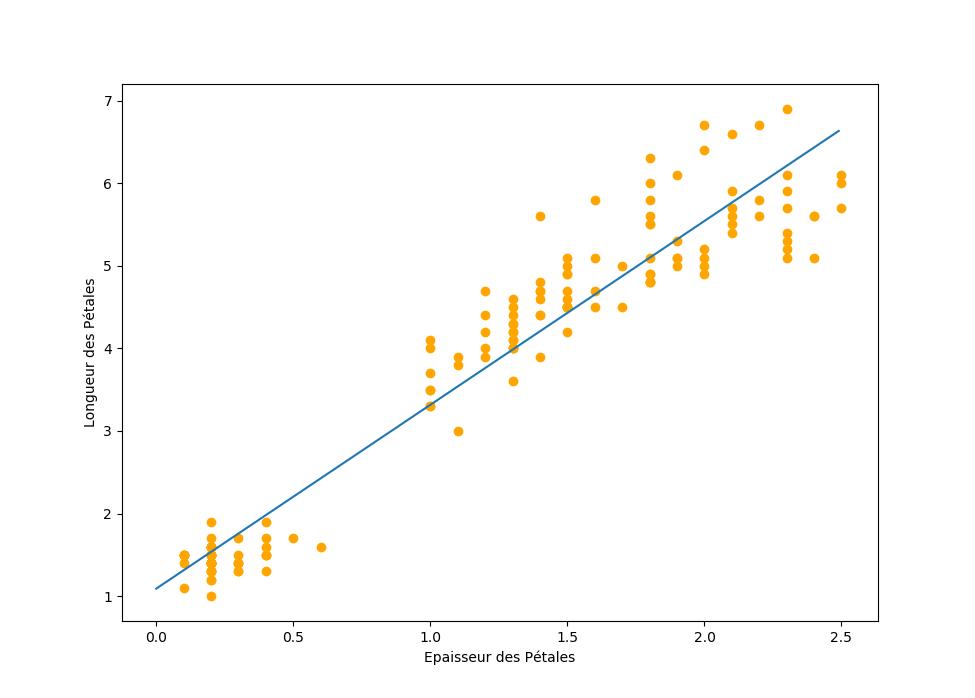
\includegraphics[scale=0.42]{ex302}
\end{frame}

\begin{frame}{Résultat attendu (2)}
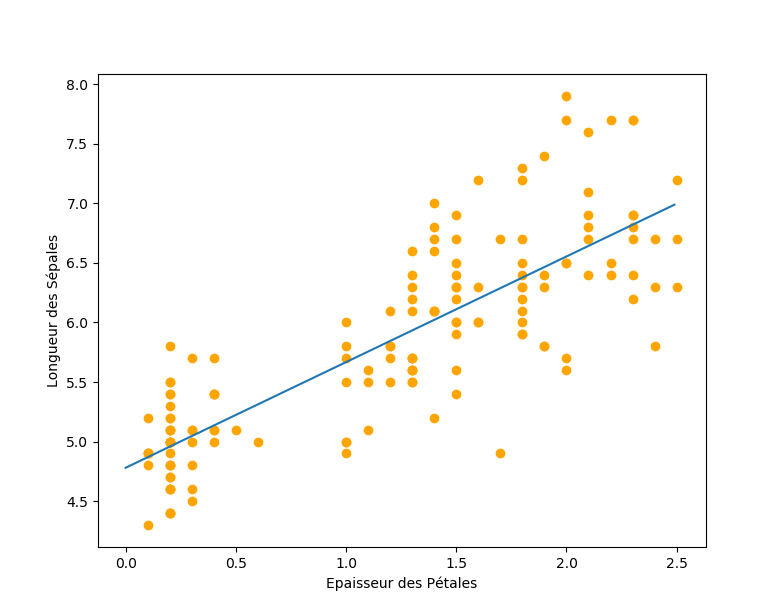
\includegraphics[scale=0.45]{ex302bis}
\end{frame}


\begin{frame}{Solution (parties 1 et 2)}
\Python{ex301}
\end{frame}

\begin{frame}{Solution (partie 3)}
\Python{ex302}
\end{frame}

\begin{frame}{Exercice}
\begin{exercice}
Importez les données de data2.csv, gardez uniquement les champs adm, dip et mil et entraînez une ACP dessus.
\end{exercice}
\begin{exercice}
Comparez graphiquement les représentations des données utilisant deux axes standards (via une scatter matrix) et celles utilisant les axes de l'ACP.
\end{exercice}
\end{frame}

\begin{frame}{Résultat attendu (1)}
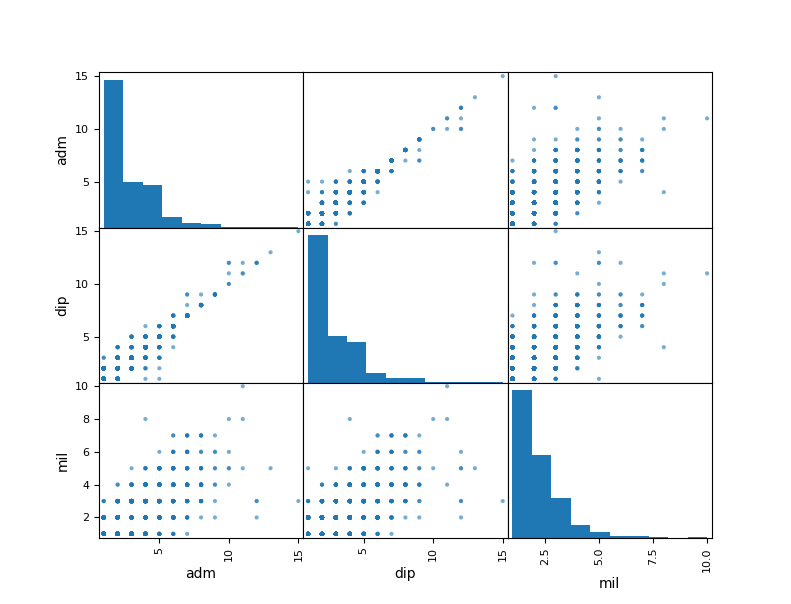
\includegraphics[scale=0.42]{ex402}
\end{frame}

\begin{frame}{Résultat attendu (2)}
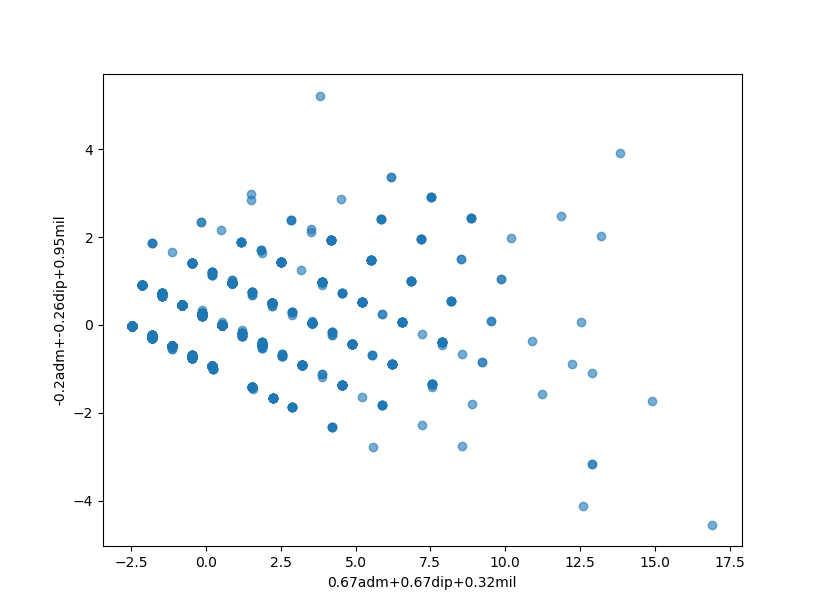
\includegraphics[scale=0.45]{ex403}
\end{frame}


\begin{frame}{Solution (partie 1)}
\Python{ex401}
\end{frame}

\begin{frame}{Solution (partie 2)}
\Python{ex402}
\end{frame}

\begin{frame}{Solution (partie 3)}
\Python{ex403}
\end{frame}



\end{document}